\documentclass{scrreprt}
\title{Building a WebGL Orrery}
\author{\textbf{Student ID:} 110059875}
\date{2014-11-21 23:59}

\usepackage{tocbibind}
\usepackage{hyperref}
\usepackage{siunitx}
\usepackage{graphicx}
\usepackage{svg}
\usepackage{float}

\begin{document}
\maketitle

\pagenumbering{roman}

\abstract{\addcontentsline{toc}{chapter}{Abstract} Building an interactive Orrery to show relationship between the Sun, planets, moons and celestial bodies within the solar system using WebGL and JavaScript. Utilising Phong shading with ambient, diffuse and specular terms. Alpha blending modes, to layer clouds over the Earth, and add rings to Saturn. Customisable parameters for the scene including camera position, zoom, field of view, simulation speed, and lighting attributes such as colour and position.

\vspace{3\baselineskip}

\begin{figure}[H]
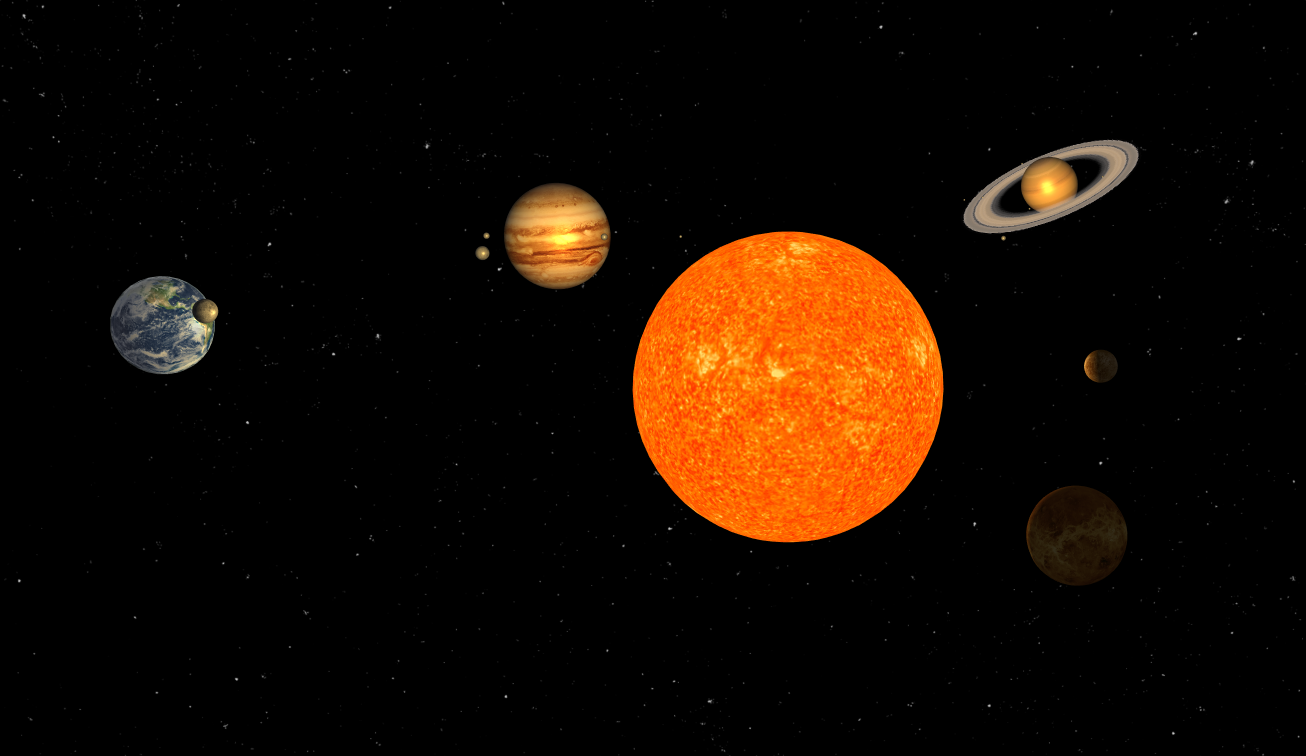
\includegraphics[width=\textwidth]{images/finished-result.png}
\caption{An image of the finished result.}
\end{figure}

}

\tableofcontents
\listoffigures

\chapter{Introduction}
\pagenumbering{arabic}
WebGL is a relatively recent\cite{khronoswebglspec} JavaScript API based on OpenGL ES 2.0 by the Khronos Group for producing interactive 3D and 2D graphics from a web browser, without any additional or proprietary plug-ins. WebGL utilises the power of graphics processing units in today's computers to provide a rich and accessible experience for 3D graphics.

WebGL was intended to be used by developers creating abstractions on-top of WebGL to make easy to use graphics libraries. This also helps when writing object oriented code (OO), as WebGL takes its procedural roots from its OpenGL ancestors. However since this was for the most part a learning exercise, we were told to use only WebGL and a library for Vector and Matrix functions.

By using WebGL, we have a pretty low level way of accessing the graphics hardware to produce 3D visualisations. These visualisations can be incredibly effective in education. Things that are hard to visualise as a static 2D image on paper come alive when shown on a screen in a 3D perspective.

An interactive Orrery can be great at showing students how orbital systems work. Especially when showing hard to visualise systems such as Saturn, with its rings and moons or Uranus, with its \ang{98} axial tilt.

To get more realistic results, we can use texture mapping to paint the surfaces of the spheres, use Phong shading to get a representation of a realistic light model with ambient lighting, diffuse shading, specular reflections.

\chapter{Methods}

The project was started by first setting up a Git repository. This is a vital first step in every single piece of work I undertake. It ensures I can easily get back to any point in time for my entire codebase. I can create branches to experiment, and track exactly how long I'm spending doing what and when.

I had to set up my project structure. All of the WebGL tutorials that I could find were strictly procedural. There was no OO influence in the code, and it was a little hard to follow as it was vastly different than what I was used to when using Java. I started out by creating a nice structure to load the canvas and WebGL context in a nice modular manner.

From there I created a scene class, which contains all the necessary information about a scene. In here, I had two loops, update and draw. Draw was looped using the requestAnimationFrame API to let the browser decide when to draw frames. This has a nice benefit of pausing when the tab is not active, reducing the load on the computer when not needed.

The update cycle is ran using setTimeout which runs every 16.667ms, which works out at 60 frames per second (FPS). By using setTimeout, the positions of planets can update consistently. However if the update cycle is too computationally complex, it will not slow down the drawing aspect of the application in any way. You can still pan around and zoom at a smooth 60FPS.

Next was choosing a library to add in support for vectors and matrices in JavaScript. For this, I used glMatrix\cite{glmatrix}, which has been in development since mid-2010 and provides over 4000 lines to provide many vector and matrix operations.

I then utilised tutorials found on WebGL Academy\cite{webglacademy} and Learning WebGL\cite{learningwebgl} to slowly build up my application from scratch. I found the WebGL Academy tutorials especially helpful, as it offered a step by step approach to programming using WebGL and explained things very thoroughly, which made it easy to adapt the code into my OO model.

To build up a scene, I decided to have an array of objects, and for each object in the array, iterate through and run their respective update and draw methods.

Building up meshes to get spheres was interesting. I had to start with triangles, then squares, and then cubes before I could create a sphere. The jump from a cube to a sphere was actually probably one of the bigger hurdles in the project, especially getting the normal maps working correctly once I had implemented lighting.

I also by accident, discovered I could create a skybox to have stars in the background of my scene. This is basically putting the entire scene inside a cube, and texturing the inside faces with stars.

Once the meshes were in place, I could focus on getting the orbits right. To do this, I needed several parameters to define a planet's movements. I needed a spin speed, axial tilt, orbit radius, orbit speed, orbit inclination and orbit offset. (See Fig. 2.1)

After getting the orbits right, texturing was really easy to do, as WebGL does most of the work for you. The textures I used were provided with the assignment spec, from NASA's Blue Marble collection\cite{bluemarblenasa} and Solar Views for the Sun\cite{solarviews}.

Directional Phong shading was one of the last things to be implemented. I started off by just having an ambient lighting term. This was an RGB value multiplied by the surface texture's RGB value. Diffuse was done by multiplying by the dot product of the normal vector, and the light direction vector. Specular was added by multiplying by the reflection vector of the normal, the view vector and a constant.

Once the directional phong was implemented, it was just a case of turning it into a point light by normalising the light position, minus the view position.

Finally as a quick addition, a loading screen was added to ensure that textures don't pop into place when loading. There's a spinner and also some helpful instructions displayed while the textures are loading.

\begin{figure}[H]
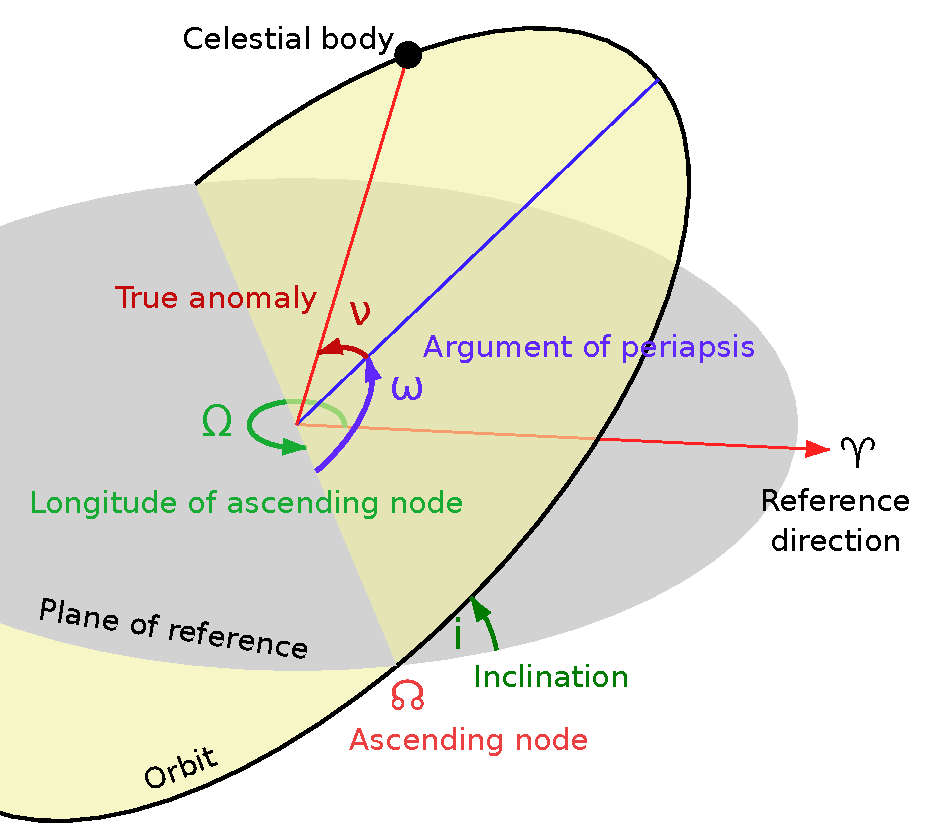
\includegraphics[width=\textwidth]{images/orbital-elements}
\caption{A diagram of orbital elements.\cite{orbitalelements}}
\end{figure}

\chapter{Results}

This project turned out very well. I had managed to do most of the things I set it out to do. I exceeded the expectations of the specification and although I didn't manage everything (orbit paths, etc. discussed in the next section) I am happy with the overall result. It's visually impressive, and is fun to play around with. I think it serves as a good visual model for how the solar system's orbits work relative to each other.

\begin{figure}[H]
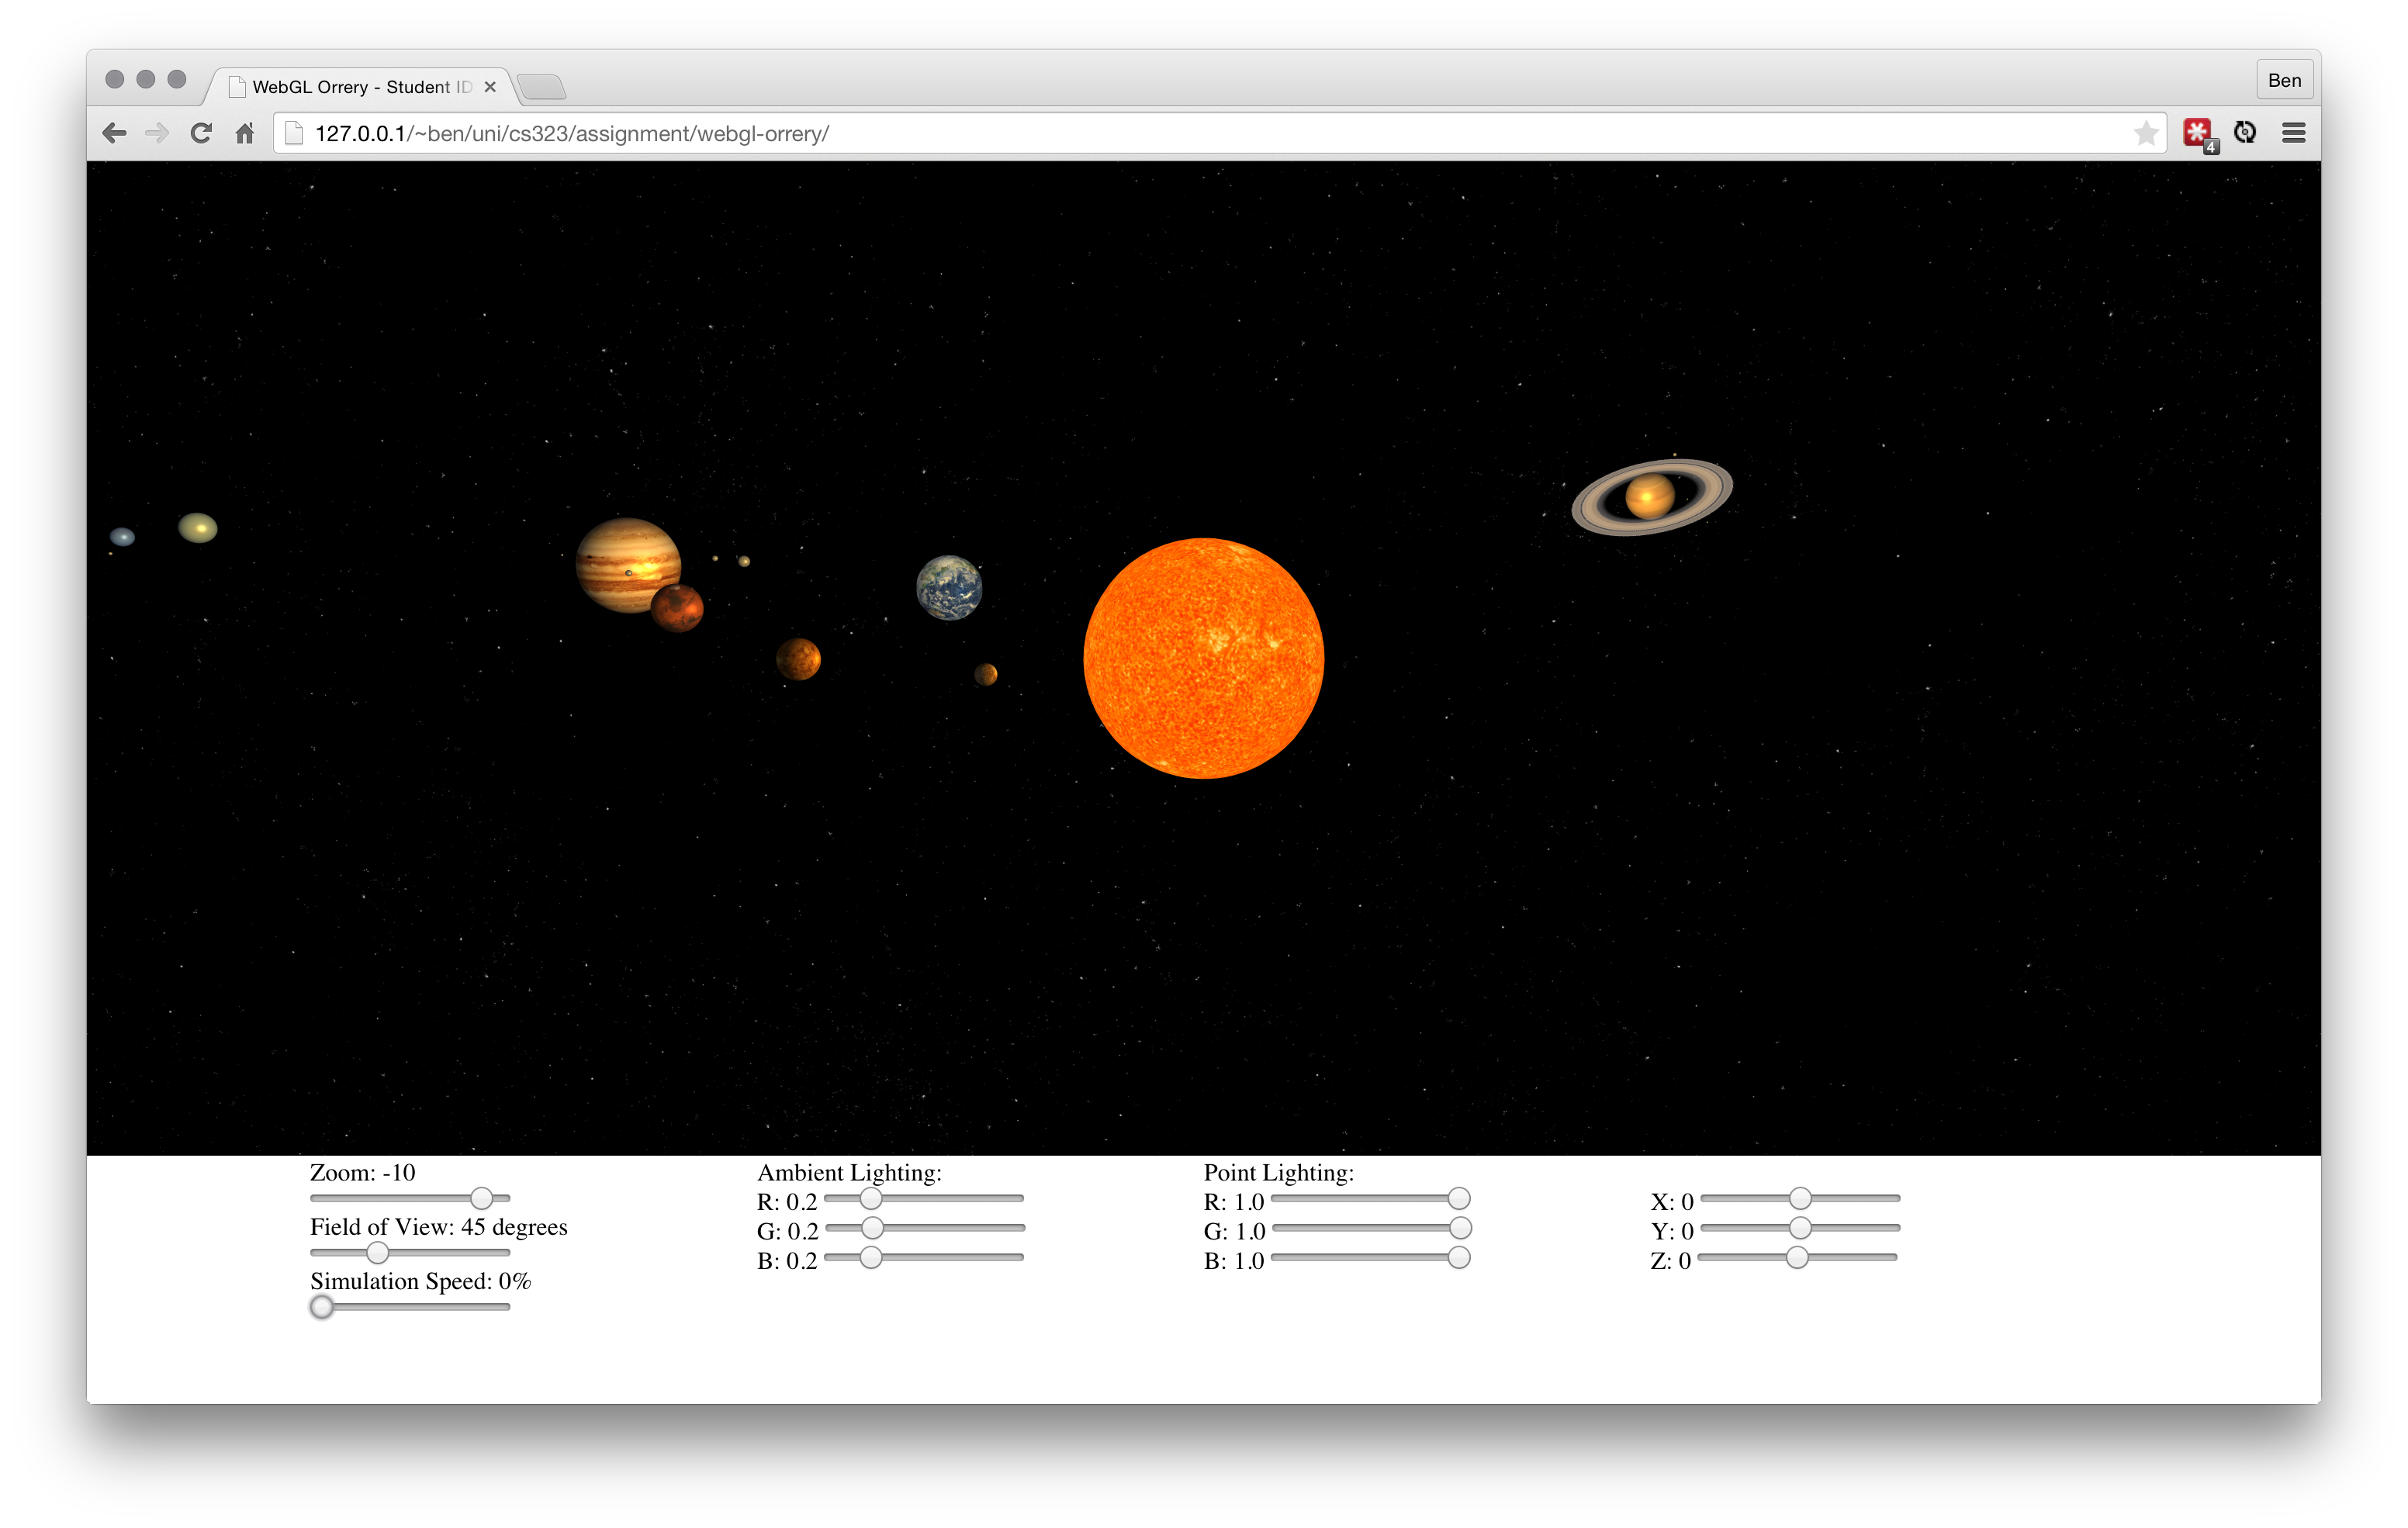
\includegraphics[width=\textwidth]{images/screenshot}
\caption{A screenshot of the final program.}
\end{figure}

As you can see, the controls on the bottom of the page let the user modify lots of things in the scene. This keeps the program from getting stale too fast, and is fun to play around with, especially the lighting ones as you'll see a few screenshots down.

\begin{figure}[H]
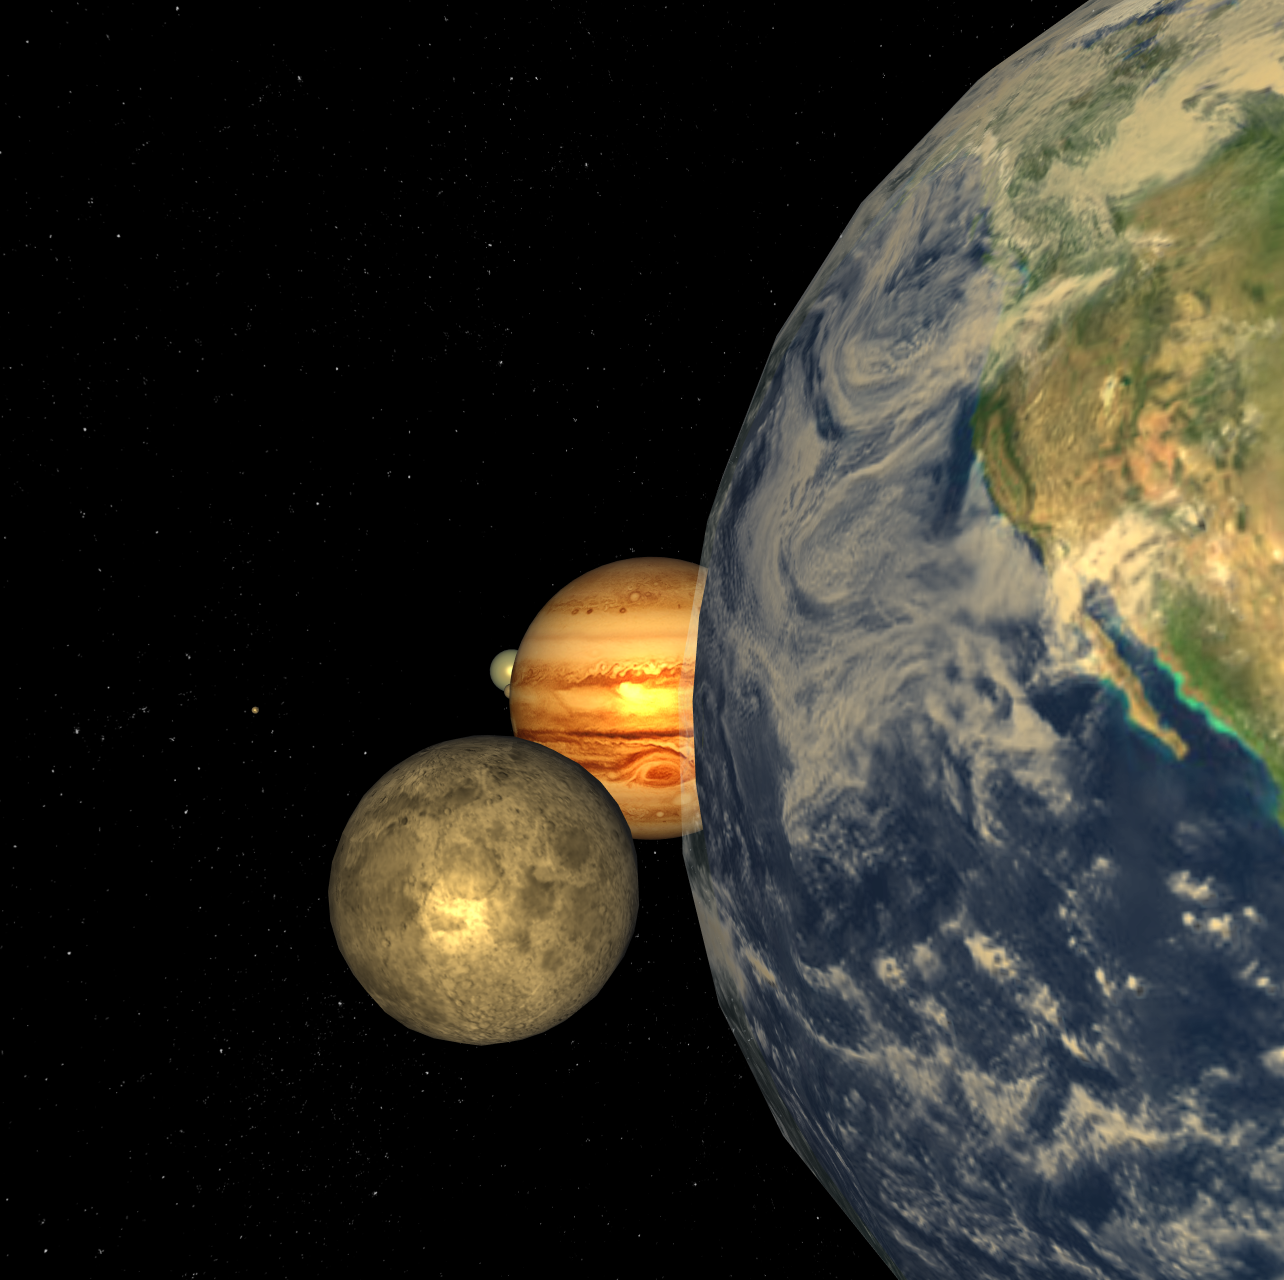
\includegraphics[width=\textwidth]{images/earthcloseup}
\caption{A closeup of the Earth, showing a cloud layer and Phong shading}
\end{figure}

The two layers of the earth are visible in this picture. You can clearly see the cloud layer floating on top of the earth as they would in real life. The polygon could of the sphere could have perhaps been a bit higher here to help with the looks.

\begin{figure}[H]
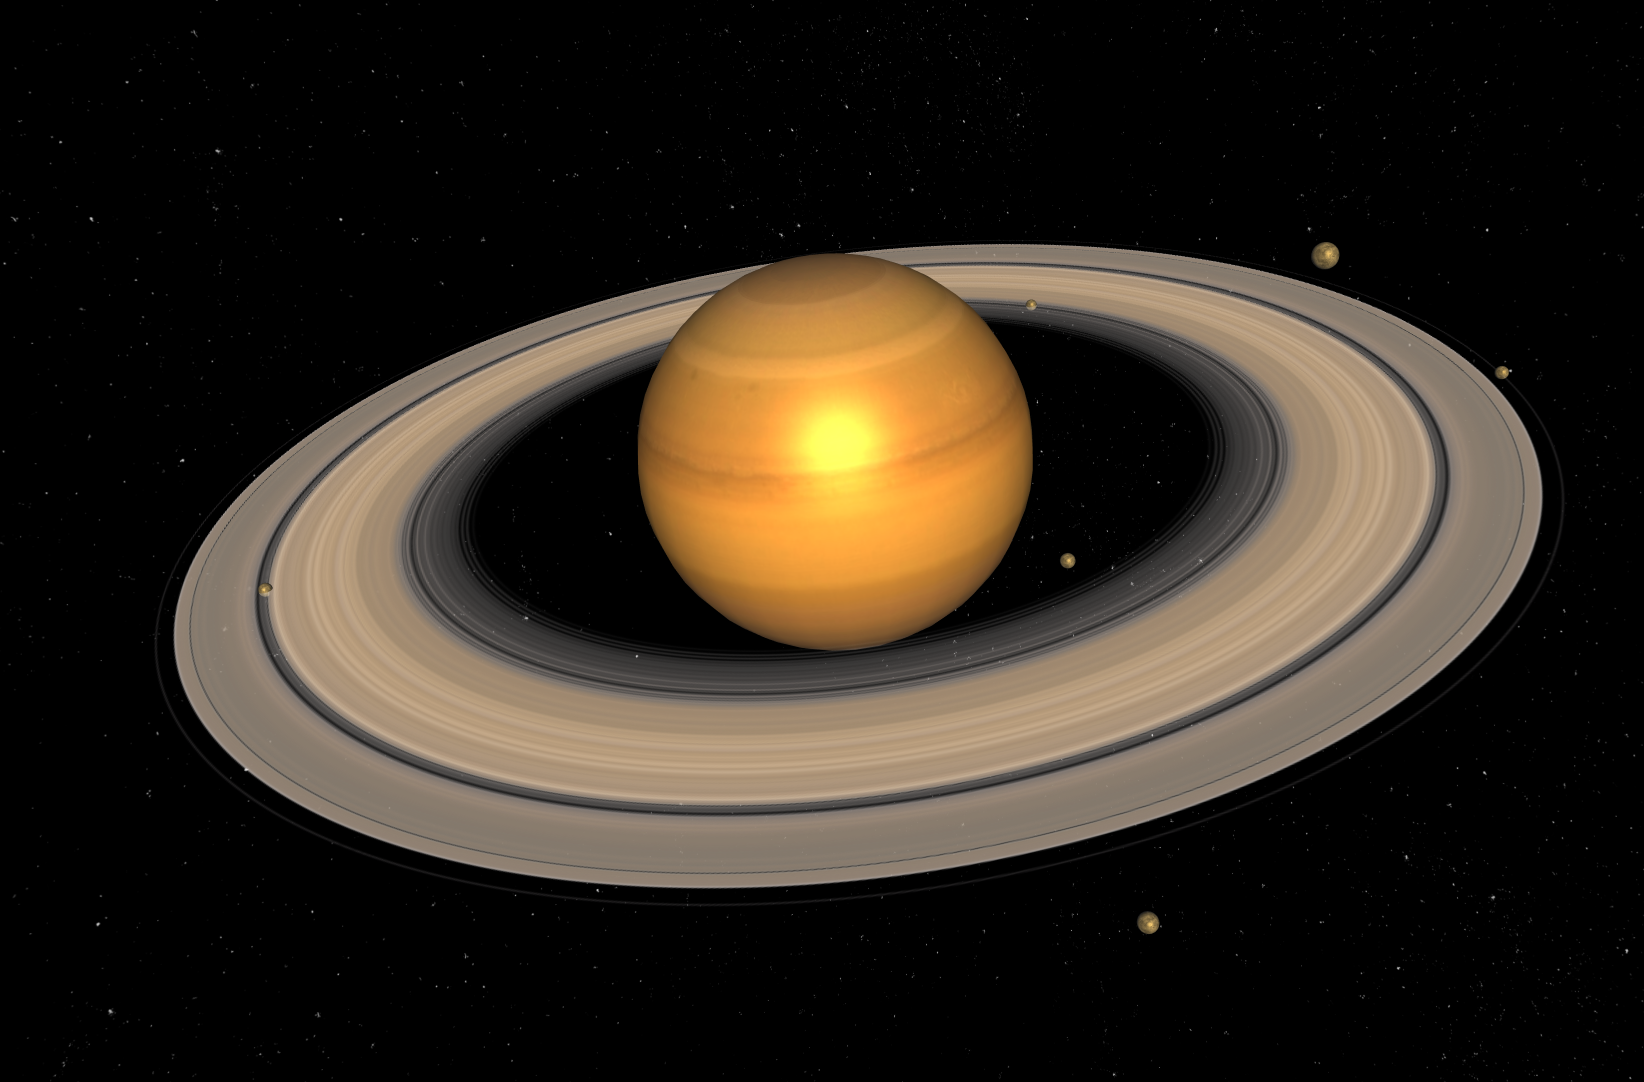
\includegraphics[width=\textwidth]{images/saturncloseup}
\caption{A closeup of Saturn and its rings.}
\end{figure}

Properly alpha blended, the stars in the background are visible through the rings.

\begin{figure}[H]
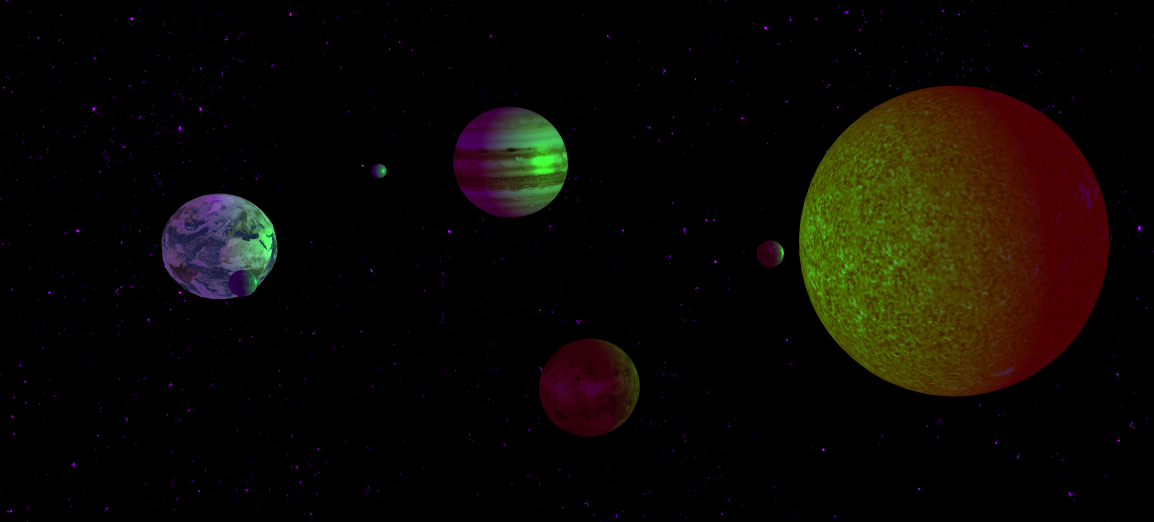
\includegraphics[width=\textwidth]{images/lighting}
\caption{A screenshot showing lighting values that have been changed.}
\end{figure}

Ambient lighting is purple, the point lighting is green with a positional offset to the left of the Sun.

\begin{figure}[H]
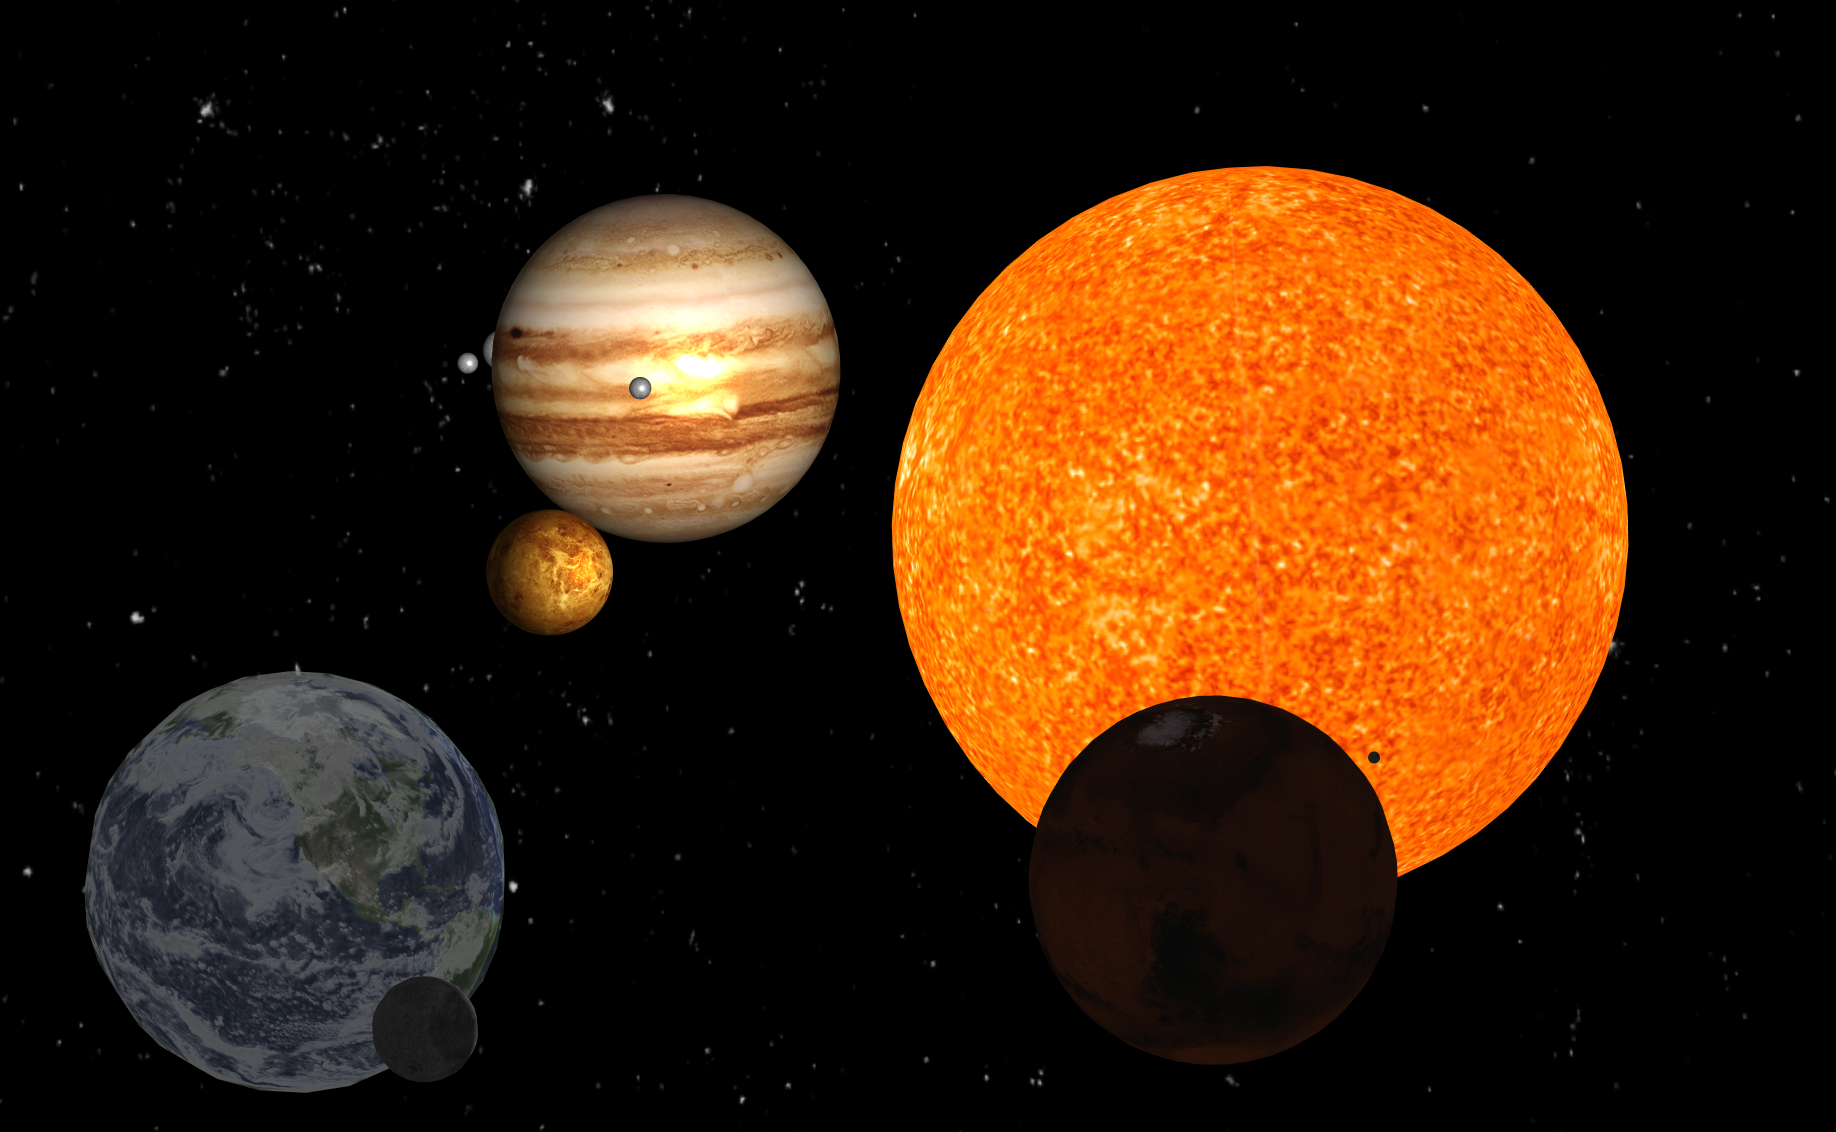
\includegraphics[width=\textwidth]{images/fov}
\caption{A forced perspective, with a low field of view and zoom.}
\end{figure}

\chapter{Discussion}

This project has many possible extensions, one of them may be to make the project include a more abstracted framework, for example having geometry classes for cubes, spheres, etc. However it could also be argued that using a framework such as three.js\cite{threejs} will accomplish this very easily.

More features include elliptical orbits, which I did not get around to implementing, lines showing the paths of the orbits, or even n-body simulation, so that changing the mass of an object has an affect on other objects.

A very nice visual effect that could enhance the looks of this project could be a basic lens flare from the sun, bloom or a glow.

Bump mapping or normal mapping the surface of planets could greatly enhance the effect that Phong lighting gives on the surfaces.

jsOrrery\cite{buildingjsorrery} implements a lot of these ideas and it is a really impressive application of WebGL.

\chapter{Conclusion}

In conclusion, if I were to write something similar again. I would definitely use a library such as Three.js to help with the abstraction of WebGL. However the project has clearly not been unsuccessful. I was able to create a nice looking approximation of the solar system, along with interactive controls and advanced shading features.

\chapter{Acknowledgments}

I would like to acknowledge M. Foskett for the help on 3D graphics concepts and for lending me three (ancient) books on 3D graphic theory. These really helped my understanding, despite being old as the concepts have pretty much remained the same. The only difference being that old methods can now be achieved in real-time.\cite{computergraphicsprinciplesandpractice}\cite{graphicsgems}\cite{three-dimensionalcomputergraphics}

\chapter{Appendices}

All project code and commit history will be publicly available through GitHub shortly after the submission deadline at the following address.

\url{https://github.com/bbrks/webgl-orrery}

A hosted demo of the project can also be found at the following URL, however this code may not represent the submitted state of the project, and may be either outdated or updated after the submission deadline.

\url{http://dev.bbrks.me/orrery}

\begin{thebibliography}{9}

    \bibitem{khronoswebglspec}
        Khronos Group (2011, Mar. 3). ``Khronos Releases Final WebGL 1.0 Specification''. Khronos Group [Online].
        Available: \url{https://www.khronos.org/news/press/khronos-releases-final-webgl-1.0-specification}. [Accessed: Nov. 21, 2014].

    \bibitem{glmatrix}
        B. Jones \& C. MacKenzie. ``glMatrix - Javascript Matrix and Vector library for High Performance WebGL apps''. glMatrix [Online].
        Available: \url{http://glmatrix.net}. [Accessed: Nov. 21, 2014].

    \bibitem{webglacademy}
        X. Bourry. ``WebGL Academy''. WebGL Academy [Online].
        Available: \url{http://webglacademy.com}. [Accessed: Nov. 21, 2014].

    \bibitem{learningwebgl}
        G. Thomas. ``The Lessons''. Learning WebGL [Online].
        Available: \url{http://learningwebgl.com/blog/?page_id=1217}. [Accessed: Nov. 21, 2014].
        
    \bibitem{orbitalelements}
        Wikipedia. ``Orbital Elements''. Wikipedia [Online].
        Available: \url{http://en.wikipedia.org/wiki/Orbital_elements}. [Accessed: Nov. 21, 2014].

    \bibitem{bluemarblenasa}
        NASA. ``Blue Marble Collections''. NASA Visible Earth [Online].
        Available: \url{http://visibleearth.nasa.gov/view_cat.php?categoryID=1484}. [Accessed: Nov. 21, 2014].
        
    \bibitem{solarviews}
        Solar Views. ``Artistic Cylindrical Map of the Sun''. Views of the Solar System [Online].
        Available: \url{http://solarviews.com/cap/sun/suncyl1.htm}. [Accessed: Nov. 21, 2014]
        
    \bibitem{threejs}
        three.js. ``three.js - Javascript 3D library''. three.js [Online].
        Available: \url{http://threejs.org}. [Accessed: Nov. 21, 2014].

    \bibitem{webglcheatsheet}
        Khronos Group. ``WebGL 1.0 API Quick Reference Card''. Khronos Group [Online].
        Available: \url{https://www.khronos.org/files/webgl/webgl-reference-card-1_0.pdf}. [Accessed: Nov. 21, 2014].

    \bibitem{buildingjsorrery}
        M. V\'{e}zina. ``Building jsOrrery, a Javascript / WebGL Solar System''. La Grange Lab [Online].
        Available: \url{http://lab.la-grange.ca/en/building-jsorrery-a-javascript-webgl-solar-system}. [Accessed: Nov. 21, 2014].

    \bibitem{computergraphicsprinciplesandpractice}
        J. Foley, et al., \textit{Computer Graphics Principles and Practice Second Edition}. Addison Wesley, 1995.

    \bibitem{graphicsgems}
        A. Glassner, \textit{Graphics Gems}. Academic Press, 1994.

    \bibitem{three-dimensionalcomputergraphics}
        A. Watt, \textit{Fundamentals of Three-Dimensional Computer Graphics}. Addison Wesley, 1989.

\end{thebibliography}

\end{document}
